\documentclass{uoyths}



%\usepackage[style=ieee,backend=bibtex]{biblatex}
\usepackage{graphicx}
\usepackage{epstopdf}
\usepackage{booktabs}
\usepackage[cmex10]{amsmath}
\usepackage{array}
\usepackage{gensymb}
\usepackage{hyperref}
\usepackage{siunitx}
\usepackage[toc,acronym]{glossaries}
\usepackage{xr}
\usepackage{listings}
\usepackage{algorithm2e}
\usepackage{gensymb}
\usepackage{textcomp}
% \usepackage[obeyspaces]{url} 
\makeglossaries

\usepackage{xcolor}
\definecolor{mygray}{rgb}{0.4,0.4,0.4}

% \lstset{
% numbers=left,
% numbersep=5pt,
% numberstyle=\tiny\color{mygray},
% showspaces=false,
% showstringspaces=false,
% tabsize=2,
% basicstyle=\footnotesize\ttfamily,
% keywordstyle=\bfseries\color{green!40!black},
% commentstyle=\itshape\color{purple!40!black},
% identifierstyle=\color{blue},
% stringstyle=\color{orange}
% }


\definecolor{mygreen}{RGB}{28,172,0} % color values Red, Green, Blue
\definecolor{mylilas}{RGB}{170,55,241}

\lstset{
    basicstyle=\small,
    breaklines=true,%
    morekeywords={matlab2tikz},
    keywordstyle=\color{blue},%
    morekeywords=[2]{1}, keywordstyle=[2]{\color{black}},
    identifierstyle=\color{black},%
    stringstyle=\color{mylilas},
    commentstyle=\color{mygreen},%
    showstringspaces=false,%without this there will be a symbol in the places where there is a space
    numbers=left,%
    numberstyle={\tiny \color{black}},% size of the numbers
    numbersep=9pt, % this defines how far the numbers are from the text
    emph=[1]{for,end,break},emphstyle=[1]\color{red}, %some words to emphasise
    %emph=[2]{word1,word2}, emphstyle=[2]{style},    
}

%\addbibresource{references.bib}

\usepackage{url}

% correct bad hyphenation here
\hyphenation{op-tical net-works semi-conduc-tor}

\usepackage{xspace}

%Glossary terms
\newacronym{ADC}{ADC}{Analogue to Digital Converter}
\newacronym{CAD}{CAD}{Computer Aided Design}


\begin{document}


% Title Page
\begin{titlepage}[cover=true, title=true, logo=true] 
\title{Autopilot for Aerial Photography}
\author{Alexander Cash}
\date{\today}
\supervisors{Dr Andrew Pomfret and Tim Clarke}
\academicyear{2015/2016}
\end{titlepage}

% Front Matter
\begin{frontMatterEnv}

% Dedication
\begin{chapterEnv}{Dedication}
Dedication
%TODO: Acknowledgements
\end{chapterEnv}

% Acknowledgments
\begin{chapterEnv}{Acknowledgements}
Acknowledgements
%TODO: Acknowledgements
\end{chapterEnv}

% ************************** Thesis Abstract *****************************
% Use `abstract' as an option in the document class to print only the titlepage and the abstract.
\begin{abstract}
This report documents the full software development cycle used to extend an open-source autopilot product. The aim of this project was to add functionality to an existing autopilot aimed at UAVs to provide better navigation for the purposes of aerial photography. The system implemented is able to both plan a battery and time efficient route for a UAV to follow, and command a given UAV to fly it. Although both of these capabilities work well independently, this report explains the shortcomings of the system as a whole, as well as its more useful features and behaviours. 
\end{abstract}


% Table of Contents
{\singlespacing\tableofcontents}%

\listoffigures

\listoftables

\end{frontMatterEnv}


\begin{mainMatterEnv}


%******************************************************************************************************
%*********************************** First Chapter ****************************************************
%******************************************************************************************************

\chapter{Introduction}  %Title of the First Chapter
\label{intro}

% **************************** Define Graphics Path **************************

\graphicspath{{Chapter1/Figs/}}


%TODO intro here? Describe what this chapter is for; background information
%TODO discuss fahim

The rest of this chapter is aimed at providing the reader with suitable background knowledge to provide context for this project and an understanding of the working environment. The last section of this chapter will outline the motivations for this project and the resulting objectives to be tackled in this project. 

%******************************************************************************************************
%******************************************************************************************************
\section{An Introduction to Unmanned Aerial Vehicles} 
\label{intro:UAVs}

The term Unmanned Aerial Vehicle (UAV) can be used to describe any form of aircraft that does not require a pilot on board. This term includes aircraft that are controlled remotely, autonomous vehicles capable of navigating themselves, and any aircraft that are a combination of the two. Other terms that may be familiar are ``drone'' and Unmanned Aerial System (UAS), which can be used interchangeably with UAV within the context of this project. 

UAVs come in a wide range of form factors but can be split into two main classes; fixed-wing UAVs and rotary wing UAVs. Fixed-wing UAVs are generally only capable of horizontal take-off and landing (HTOL), whilst rotary wing UAVs generally employ vertical take-off and landing (VTOL). There are, however, other forms of UAV which incorporate features of both main classes; for example, quadplane UAVS use rotary wing rotors to allow VTOL, but do the main bulk of their flying with forward facing rotors much like a fixed-wing UAV. Across these categories are a very wide range of UAV platforms, from hobbyist quadcopters to military attack vehicles, and many many others in between. %TODO images?  
Although the range of UAV form factors and their uses is vast, the vast majority are suitable for candidates for complete autonomous flight control, as shall be described in Section %TODO reference where we talk about adding hardware modules 
 
Although there were a large number of suitable candidates for the following work, it was decided that this project would be aimed at the control of strictly fixed-wing UAVs for the purposes of aerial photography. For that reason, we shall not discuss any other style of UAV. %TODO 

%******************************************************************************************************
%******************************************************************************************************
\section{UAVs for Aerial Photography} 
\label{intro:photography}

The first recorded use of aerial photography was in 1858 by a French balloonist and photographer known as ``Nadar'' at a height of 80 metres using a tethered hot air balloon. %TODO ref aerial photography history
Since then aerial photography has of course massively progressed, both in terms of the aerial vehicles in use and the cameras available. As such, it is now an activity that can be partaken in by both organisations, companies, and individuals alike, for a range of purposes. For example, aerial photography of course plays a very large role in intelligence gathering by government agencies and militaries, but can also be a hobby for otherwise earth-bound photography enthusiasts. 

Different applications will require different equipment and styles of photography; a hobbyist may want a wide panorama, whilst a mapping application will require a consistent vertical camera angle. The use of aerial photography for mapping or measurement is known as aerial photogrammetry, and will be the chosen field of interest for this project. Aerial photogrammetry is a specific subset of aerial photography in that it not only requires the capturing of images, but additional information about where the image was captured. For this project, we are looking at the use of aerial photogrammetry to create an image of the land below our UAV, either for mapping or general surveying purposes. In order to be able to do this, we need to be able to capture a set of images, and know the location of the UAV when the images were captured, to allow the images to be stitched together into one larger image of the ground beneath. In this scenario we can typically use GPS co-ordinates and a pre-planned imaging path to define which images relate to which areas of the ground below. %TODO refernce photogrammetry definition?


This project will primarily focus on the mapping of land beneath the UAV, and as such we need to define a specified flightpath over the chosen area. There are a number of typical flightpaths for surveying or mapping land, two forms are lawnmower pattern paths and spiral pattern paths. Fig. \ref{fig:simplelawnmower} shows the general form of a lawnmower pattern, and Fig. \ref{fig:simplespiral} shows us the general form of a spiral pattern.

\begin{figure}[htbp!] 
\centering    
\includegraphics[width=0.7\textwidth]{SimpleLawnmower}
\caption[Simple Lawnmower Pattern]{The general form of a lawnmower pattern aerial imaging flightpath}
\label{fig:simplelawnmower}
\end{figure}

\begin{figure}[htbp!] 
\centering    
\includegraphics[width=0.7\textwidth]{SimpleSpiral}
\caption[Simple Spiral Pattern]{The general form of a spiral pattern aerial imaging flightpath}
\label{fig:simplespiral}
\end{figure}

Using these patterns, we can define what shall be referred to henceforth as ``imaging paths'' or ``imaging runs''. These are the sections of the flightpath for which we are capturing images of the ground below, and as such we very much care about the position and orientation of the UAV whilst following these paths. For the lawnmower pattern the imaging paths are the vertical sections of the path seen in Fig. \ref{fig:simplelawnmower}, whereas for the spiral path all sections of the flight plan are considered imaging paths. 

As the lawnmower pattern does not require the horizontal sections of the path in Fig. \ref{fig:simplelawnmower} to be used for capturing images, we are not particularly concerned with how we fly between the imaging paths. Knowing this, we can specify our flightpath in terms of simply our imaging paths, as can be seen in Fig. \ref{fig:imaginglawnmower}

\begin{figure}[htbp!] 
\centering    
\includegraphics[width=0.7\textwidth]{ImagingLawnmower}
\caption[Imaging Lawnmower Pattern]{A version of the lawnmower pattern, using only imaging paths}
\label{fig:imaginglawnmower}
\end{figure}

As the imaging paths shown in Fig. \ref{fig:imaginglawnmower} are separate of one another, it is possible to complete each imaging path in any order and in either direction. This does however require the user to plan accordingly and to record location data accurately so as to be able to stitch together the resulting photographs correctly. One of the resulting patterns that we can create from this is called the ``Zamboni pattern'', named after the route a Zamboni machine takes around an ice rink to smooth out the ice. A Zamboni pattern describes a path whereby we d onot traverse up and then down adjacent imaging paths, but instead perform a series of overlapping paths by travelling up one imaging path, and then down a path a few rows over. This is necessary for a Zamboni due to its large minimum turning radius, and would be equivalent to a UAV with a large turning radius being required to traverse a number of very close imaging paths. 

The required flightpath will have to be calculated based on a number of factors including:
\begin{itemize}
	\item The size of the area we are wishing to photograph
	\item Changes in ground elevation over the chosen area
	\item The operational range of the UAV based on battery life or fuel amount
	\item The desired resolution of the resulting images - we must fly lower for higher detail images
	\item The distance between imaging paths will be a function of the desired flying height and the angle of the lens on the camera
	\item The path to follow between the imaging paths will be a function of the turning performance of the UAV
	\item Environmental factors such as wind during the flight
\end{itemize}

These factors shall be considered and discussed later in this report where relevant, and have been used to inform decisions throughout the work of this project.

Throughout this work we shall be referring to a flightpath as a ``mission'', which describes a full, pre-planned flight path from take-off to landing. To define these missions we require particular software products that shall be discussed in Section \ref{intro:planner}.



%TODO finalise
%TODO define mission planning process in this section

%******************************************************************************************************
%******************************************************************************************************
\section{ArduPilot} 
\label{intro:ardupilot}

ArduPilot, also known as ArduPilotMega (APM), is an open-source suite of autopilot products aimed at hobbyists and professionals alike. ArduPilot includes the ArduPlane, ArduCopter, and ArduRover autopilots, each aimed at aeroplane style UAVS, helicopter and multirotor UAVS, and ground based rover platforms respectively. As previously mentioned, this project is aimed at fixed-wing aeroplane UAVs, and as such this report is looking at the ArduPlane product. 

ArduPilot has been around since late 2009 and was originally designed to operate using the Arduino development ecosystem. Since then, the codebases have evolved in both size and functionality, in part due to hardware improvements which will be discussed in \ref{intro:planner}. This has lead to both the software and hardware components of these ArduPilot autopilot solutions moving away from Arduino almost entirely.

ArduPilot grew out of an organisation called DIYDrones, %TODO ref DIYDrones.com
which was set up as an online community for enthusiasts to discuss and create solutions for UAV use; this community still exists and operates as one of the many hubs for discussion regarding UAVs, autopilots, and route planning. In 2014, the group of people maintaining the ArduPilot project teamed up with The Linux Foundation to create a non-profit organisation called the Dronecode Project. The Dronecode Project is an effort to collaborate a number of open-source hardware and software products under one structure, which includes the ArduPilot project. In February 2016, it was announced that the core team behind ArduPilot would be creating their own non-profit organisation to best suit the needs of the users of the ArduPilot products, however at the time of writing this is still a work in progress. %TODO ref dronecode, non-profit announcements, linux foundation

\subsection{ArduPlane}
\label{intro:arduplane}

ArduPlane is designed so that when paired with a suitable controller board (see Section \ref{intro:hardware}), it enables autonomous flight on almost any fixed-wing UAV. %TODO ref http://ardupilot.org/plane/index.html 
To do this, the ArduPlane software is compiled to create the firmware, which is then programmed onto the controller board alongside the mission plan. Once the controller board is connected to all of the necessary control outputs and sensor inputs, the UAV must be configured and tuned for flight, and then is ready for take-off. The configuration and tuning are of course capabilities provided by ArduPlane, however are not relevant for discussion within the context of this project. ArduPlane handles both automatic take-off and landings, as well as providing the option to change between flight modes. The flight modes available include fly-by-wire modes, an acrobatics mode, a training mode, and an automatic flight mode. For this project we are only concerned with the automatic flight mode, and shall not be dealing with any other mode. 

The ArduPlane codebase uses a very large collection of libraries, of which the majority are also used by the ArduCopter and ArduRover products. This, combined with the fact that ArduPlane is designed to work with any fixed-wind UAV means that a lot of the code is very generic and reusable. The codebase for the whole ArduPilot project currently consists of roughly 11,000 files in total, and the specific ArduPlane code (excluding any shared libraries or resources) is made up of only 37 files. The sheer number of shared files, generic coding style, and open-source nature of this project combine to mean that in many respects the code commenting and documentation is very lacking and unspecific. That being said, there are a number of instructional guides and references that can be found on the ArduPilot website for anyone looking to modify the code or get involved with contribution. In addition to this, there are a number of forums that can provide many answers to common problems. %TODO ref diydrones, discuss.ardupilot.org, and apm forum	
In addition to there being three main autopilot platforms, there are also a large number of differing released versions and code branches, which are often platform specific or hardware specific.

%TODO finish?


\subsection{JSBSim}
\label{intro:jsbsim}

As the ArduPilot project is open source, there are a number of associated open-source utilities available to download for testing purposes. One of the main tools used in ArduPlane development is called JSBSim, an open-source Flight Dynamics Model (FDM) which can be used as part of a flight simulator. %TODO ref jsbsim.sourceforge.net

We are able to use this FDM to provide a Software In The Loop (SITL) simulator, which does not require any additional hardware besides a computer. This enables us to modify the ArduPilot code and test it with a range of flight missions without the need to purchase a control board or have a suitable UAV available. 

The ArduPlane project includes a utility to simulate and view a fixed-wing UAV in flight, starting at any given GPS location. Fig. \ref{fig:jsbsim} shows one example of this, where we have the command window, an output console, and a map view. The map view shows us the planned mission and the actual path the UAV will follow in the given scenario, the console window displays output and communication messages from the UAV, and the command window allows us to control the simulator.

\begin{figure}[htbp!] 
\centering    
\includegraphics[width=\textwidth]{JSBSim}
\caption[JSBSim Simulator]{A view of the JSBSim based flight simulator, showing a command window, output console, and simulator map view}
\label{fig:jsbsim}
\end{figure}

This simulator forms the bulk of the testing for this project, and is used to map flight paths and record performance. Each simulated UAV flight generates a log in the form of a \textit{.BIN} file. We can then use the MAVExplorer utility and our ground control software to analyse the log files. 

\subsubsection{MAVExplorer}
\label{intro:mavexplorer}
MAVExplorer is a log analysis tool, provided in the form of a python script suitably named \textit{MAVExplorer.py}. This allows us to generate a map of the area over which the UAV has flown with white lines displaying the planned mission, and a green line plotting the actual route the UAV flew. An example of this can be seen in Fig. \ref{fig:mavexplorer}.

\begin{figure}[htbp!] 
\centering    
\includegraphics[width=\textwidth]{MAVExplorer}
\caption[MAVExplorer Example]{The mapping view provided by MAVExplorer utilising log files from flight simulations}
\label{fig:mavexplorer}
\end{figure}

\subsection{MissionPlanner and APM Planner}
\label{intro:planner}

As previously mentioned, for autonomous UAV flight we need to plan out a mission before flight. There are a number of software products capable of this, however the main two used by the ArduPilot project are called APM Planner 2 and MissionPlanner. Both of these products are open source however APM Planner 2 runs on Linux, Windows, and Mac OSX, whilst MissionPlanner is a Windows only application. Both products enable mission planning however the MissionPlanner product is more feature rich, reliable, and quick to use. 

The missions plans generated using either of these programs are of the same format; a text file with a number of commands, parameters, and often GPS locations. This is very useful as it allows manual editing of these text files where necessary, and allows us to easily work out how the autopilot itself reads its commands from the provided mission plan. 

There are a wide range of commands that can be included in a mission including take off commands, land commands, and navigation commands. For this project the most relevant navigation commands are those conducted using waypoints. We are able to instruct he UAV to loiter around a point at a specified radius for a number of rotations (complete circles around a point), a duration, or indefinitely. The other form of navigation command is simply an instruction to travel to a point in space, with the option to define how close to that point we need the UAV to travel. 

Fig. \ref{fig:missionplanner} shows a typical mission plan in MissionPlanner, where we are commanding a simple lawnmower pattern imaging run. 

\begin{figure}[htbp!] 
\centering    
\includegraphics[width=\textwidth]{MissionPlanner}
\caption[MissionPlanner Desktop Software]{The mission planning view of the Windows based MissionPlanner software}
\label{fig:missionplanner}
\end{figure}

%******************************************************************************************************
%******************************************************************************************************
\section{Autopilot Hardware} 
\label{intro:hardware}

As also mentioned, one of the key components for autonomous UAV flight using ArduPlane is the controller board which must be mounted on the UAV itself. There are a number of currently available boards that ArduPilot can run on, and over the years there have been many versions of these. These control boards are responsible for processing the mission plan and controlling the aircraft accordingly. During flight, the control board uses GPS readings alongside other sensor readings where available to direct the aircraft. It does this using the servos connected to the control surfaces, and controlling the thrust generated from the propeller(s) or engine(s). The control board can be connected other devices too, such as camera gimbals and parachute release devices, however these are not in use throughout this project. 

There are currently 4 supported controller boards that have open hardware design, and 4 controller boards with closed hardware designs. Additional to this are a number of controller boards which are no longer supported, as they do not have the storage capabilities to load on the latest versions of the code. The most popular currently supported board is the Pixhawk board, which can be seen in Fig. \ref{fig:pixhawk}, and has an open hardware design. The APM 2.x series of controller boards, seen in Fig. \ref{fig:apm2}, used to be very popular however are no longer supported for the latest versions of the code.

\begin{figure}[htbp!] 
\centering    
\includegraphics[width=0.6\textwidth]{Pixhawk}
\caption[Pixhawk Controller Board]{The Pixhawk controller board, for which the hardware specification and design is openly available, from \cite{Pixhawk}}
\label{fig:pixhawk}
\end{figure}

It is possible to still use the APM 2.x boards as they are still available for purchase online and will work with older versions of the ArduPlane code. This may be beneficial in certain situations, as the Pixhawk board is considerably more expensive than an APM board. The presence of a controller board is not essential for this project, as we are able to use the SITL simulator described in Section \ref{intro:jsbsim} to simulate UAV flight without one. If one is present, it is possible to use a Hardware In The Loop (HITL) simulator to test changes to the codebase by running them on a controller board. In this instance, the controller board replaces JSBSim whilst simulating flight.

\begin{figure}[htbp!] 
\centering    
\includegraphics[width=0.5\textwidth]{APM2}
\caption[APM 2.6 Controller Board]{The APM 2.6 controller board, which is no longer supported by the ArduPilot project, from \cite{Apm2}}
\label{fig:apm2}
\end{figure}

%******************************************************************************************************
%******************************************************************************************************
\section{Project Motivations and Objectives} 
\label{intro:objectives}

The inspiration for this project comes from its supervisor, Dr Andrew Pomfret. He was part of an expedition to map a glacier in Svalbard, Norway using a UAV equipped with a camera in order to determine any movement of the glacier over time. Although using a professional grade UAV and associated route planning software, he found a number of its features lacking. The most relevant issue was that planning a battery efficient route that would also capture high quality images was laborious, and that regardless of how well you planned the route, he felt the UAV would often not be optimising its battery usage. Following lengthy discussion between the author and Dr Pomfret, two primary objectives were defined.

\subsection{Objective 1: Efficient Route Planning}
\label{intro:obj1}
Our first objective is to implement an efficient method for route planning. The solution should enable a user to plan a route that allows us to deliver high quality aerial photographs, without using more battery power than is required. When discussing high quality aerial photographs, we are talking primarily about the position of the UAV relative to the planned route above ground, and as such we require the UAV to be commanded to follow the imaging paths described in Section \ref{intro:photography}. This requires us to plan a route which will result in the UAV travelling the full length of the imaging path which in turn requires the UAV to be aligned with the imaging path before starting it. 

A further requirement for this task is that the planning method should be user-friendly and calculate a desired route from standard waypoint definitions provided in the mission planning software.

Building on these aims, it is necessary for this system to work for flight in any environment, meaning it must be able to plan a route that works for the UAV in windy conditions. As such we must incorporate knowledge of the flying environment when planning the path, be that in real-time when flying or beforehand when plannig, this shall be explored later.

\subsection{Objective 2: Route Following}
\label{intro:obj2}

Our second objective follows on from our first objective, and requires us to enable the UAV to fly the newly define path types. This will require modification of the ArduPlane code so as to be able to understand any new commands and perform them as desired. This may also require a new method of path following than is currently available in official versions of ArduPlane. 

Additionally, this objective should work with the first to provide flight in windy conditions. This may be entirely a feature of the planning stage or it may be a feature of the autopilot implementation, this shall be explored later.
%TODO finalise objectives


%******************************************************************************************************
%****************************** Second Chapter ********************************************************
%******************************************************************************************************

\chapter{Literature Review}
\label{litrev}

% **************************** Define Graphics Path **************************
\graphicspath{{Chapter2/Figs/}}
% **************************** Define Graphics Path **************************

Now that we have clearly defined objectives, it is necessary to discuss and analyse existing literature that may help to understand and complete our aims.  
%TODO introduce sectino properly


%******************************************************************************************************
%******************************************************************************************************
\section{Dubins Paths}
\label{litrev:dubins}
In 1957, an American mathematician by the name of Lester Dubins 


\begin{figure}[htbp!] 
\centering    
\includegraphics[width=0.5\textwidth]{LSL}
\caption[Dubins LSL Path]{}
\label{fig:lsl}
\end{figure}

\begin{figure}[htbp!] 
\centering    
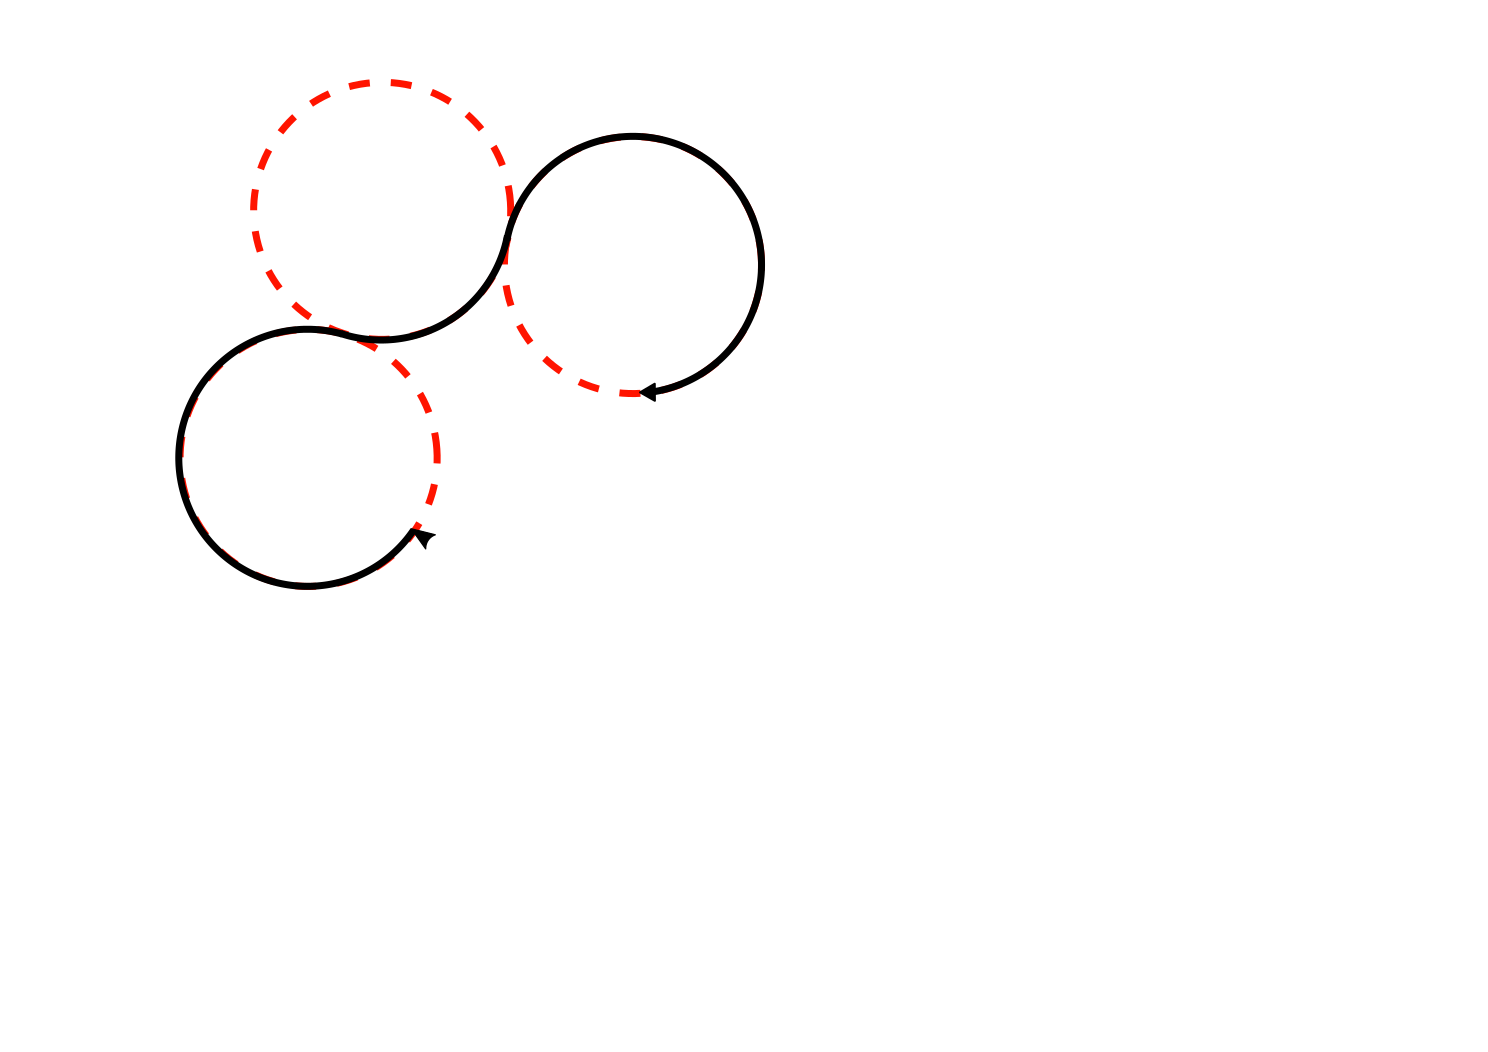
\includegraphics[width=0.5\textwidth]{RLR}
\caption[Dubins RLR Path]{}
\label{fig:rlr}
\end{figure}

\begin{figure}[htbp!] 
\centering    
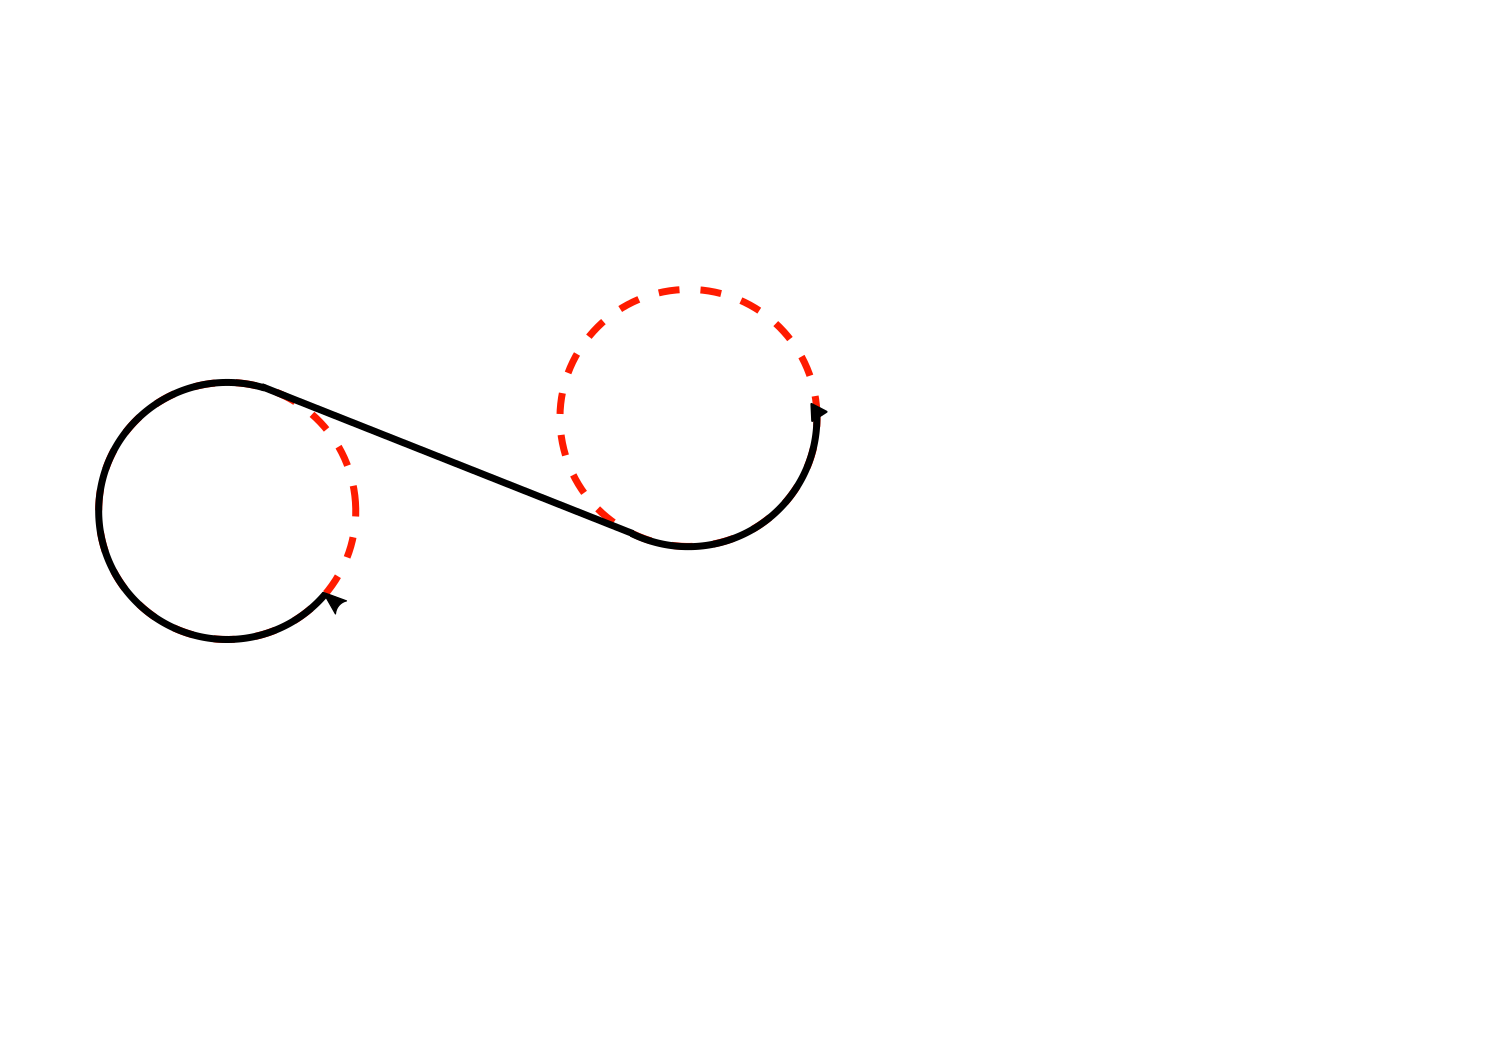
\includegraphics[width=0.5\textwidth]{RSL}
\caption[Dubins RSL Path]{}
\label{fig:rsl}
\end{figure}

%******************************************************************************************************
%******************************************************************************************************
\section{Path Following in Wind}
\label{litrev:path}

%******************************************************************************************************
%******************************* Third Chapter ********************************************************
%******************************************************************************************************

\externaldocument{{../Chapter1/chapter1}}
\externaldocument{{../Chapter2/chapter2}}
\externaldocument{{../Chapter4/chapter4}}
\externaldocument{{../Chapter5/chapter5}}

\chapter{Task One: Path Planning}
\label{task1}

% **************************** Define Graphics Path **************************
\graphicspath{{Chapter3/Figs/}}

%******************************************************************************************************
%******************************************************************************************************
\section{The Problem}
\label{task1:description}


%******************************************************************************************************
%******************************************************************************************************
\section{Solution}
\label{task1:solution}


%******************************************************************************************************
%******************************* Fourth Chapter *******************************************************
%******************************************************************************************************

\externaldocument{{../Chapter1/chapter1}}
\externaldocument{{../Chapter2/chapter2}}
\externaldocument{{../Chapter3/chapter3}}
\externaldocument{{../Chapter5/chapter5}}

% **************************** Define Graphics Path **************************
\graphicspath{{Chapter4/Figs/}}


%******************************************************************************************************
%******************************************************************************************************
\chapter{Task Two: Path Following}
\label{task2}

This is the second of two tasks carried out in this project. Whilst our previous task was aimed at planning paths on the ground prior to flight, this task is aimed at commanding the UAV to fly such paths.


%******************************************************************************************************
%******************************************************************************************************
\section{Path Following - Aims}
\label{task2:aims}

The overarching aim for this task is to implement changes to ArduPlane to allow us to fly an air relative Dubins path as defined by the work already completed. Thanks to our path planning solution the UAV does not need to be aware of its ground relative location in order to successfully navigate to our desired point. The path following solution must simply interpret our description of a Dubins path and perform the desired manoeuvres. 

We need to be able to take a mission plan created using MissionPlanner or APM Planner 2 and insert a series of flight commands that will result in the UAV flying our desired Dubins path. To do this, we need to define the these commands in a format the autopulot will understand, and then enable the autopilot to respond to these input commands. 

We can summarise this tasks as being aimed at achieving the following:

\begin{itemize}
	\item Being able to describe a Dubins path using MAVLink messages %TODO introduce mavlink messages
	\item Enabling the UAV to interpret and act upon the new MAVLink messages
	\item Successfully command the UAV to fly a Dubins path, both with and without the presence of wind
	\item Successfully commanding the UAV to fly in wind to a ground relative point using a Dubins path 
\end{itemize}

From these aims, we can define a number of stages to split this task into, as we did with the previous task. Doing so simplifies design, implementation, and testing, whilst also providing clear milestones and cut off points to work well with the planning processes used in this project.These stages were defined as:

\begin{enumerate}
	\item Define the format of new commands required to fly a Dubins path
	\item Enable the UAV to interpret newly added commands
	\item Command the UAV to fly a Dubins path in both the presence and absence of wind
\end{enumerate}

%******************************************************************************************************
%******************************************************************************************************
\section{Path Following - Stage 1: Defining New Flight Commands}
\label{task2:stage1}

In this section we shall follow the design, implementation, and testing phases completed in order to define our new flight commands. This work prepares us for the next stage of adding functionality to ArduPlane so as to read, interpret, and act upon the new commands we have provided. 

\subsection{Stage 1: Design and Implementation}
\label{task2:stage1:design}

ArduPilot products use MAVLink messages to define all of the commands that may be included in a mission plan; a full list of the current MAVLink messages can be seen at \cite{MavlinkMessages}. A complete mission plan will simply be a collection of MAVLink messages, where each line corresponds to one MAVLink message, consisting of the following fields:

\begin{itemize}
	\item INDEX - an identifier for each command
	\item CURRENT WP - indicating which waypoint the command relates to (irrelevant for this project)
	\item COORD FRAME - indicates whether altitude values are relative to the takeoff altitude or to previous waypoint altitude
	\item COMMAND - the command number used to identify each instruction in the mission plan
	\item PARAM1 - optional parameter field
	\item PARAM2 - optional parameter field
	\item PARAM3 - optional parameter field
	\item PARAM4 - optional parameter field
	\item PARAM5/X/LONGITUDE - optional parameter field or a GPS longitude value 
	\item PARAM6/Y/LATITUDE - optional parameter field or a GPS latitude value
	\item PARAM7/Z/ALTITUDE - optional parameter field or an altitude value
	\item AUTOCONTINUE - flag to indicate whether to continue through the mission plan after this command
\end{itemize}

 To keep our system as simple as possible, it was decided that the easiest way to describe a Dubins path using MAVLink messages was to generate an individual message for each segment of the path. This would allow us to create a MAVLink message that indicated whether the segment needed to be a left-hand turn, right-hand turn, or a straight line. The console application created for path planning accepts the UAV's airspeed as an inpurt argument, and outputs the path as three segments and displays their length. This meant that it was very simple to create a MAVLink message indicating just two things; the segment turn direction, and the duration for the UAV to fly it. 

 As our paths had been designed independent of GPS co-ordinates, each MAVLink message only needed to include the command value, and the duration value in one of the parameter fields. We didn't need any GPS or altitude information in PARAM5, PARAM6, or PARAM7. By following the information found in the developer's wiki at \cite{ArduPilotMAVLink}, we were able to add four new commands. As we knew that our new commands were to be navigation commands, we followed the MAVLink convention of starting the names with ``MAV\_CMD\_NAV\_''. We decided to name our new messages as follows:

 \begin{enumerate}
 	\item MAV\_CMD\_NAV\_DUBIN\_LEFT
 	\item MAV\_CMD\_NAV\_DUBIN\_RIGHT
 	\item MAV\_CMD\_NAV\_DUBIN\_STRAIGHT
 	\item MAV\_CMD\_NAV\_DUMMY\_WP
 \end{enumerate}

 The last command was a dummy command, included so that we would be able to include one of these commands into a simulation, print out a message into the simulator console and therefore be confident that our commands were being read correctly by the autopilot. As the name would suggest, this final command was never intended to do anything other than provide a verification technique.

 The new message types were defined in \path{.../ardupilot/libraries/GCS\_MAVLINK/message\_definitions/ardupilotmega.xml}. This is the file where developers add platform specific commands, not intended to be shared with other ArduPilot products such as ArduCopter; this is because GCS\_MAVLINK is a shared library, in which most MAVLink messages are defined in the file \path{.../ardupilot/libraries/GCS\_MAVLINK/message\_definitions/common.xml}.

 An example of one of these definitions is as follows:

 \begin{minipage}{\linewidth}
\begin{lstlisting}[language=XML]
<entry name="MAV_CMD_NAV_DUBIN_RIGHT" value="86">
	<description>Perform a RIGHT turn segment of a dubins path turn</description>
	<param index="1">Duration of time to fly this segment</param>
	<param index="2">Empty</param>
	<param index="3">Empty</param>
	<param index="4">Empty</param>
	<param index="5">Empty</param>
	<param index="6">Empty</param>
	<param index="7">Empty</param>
</entry>
\end{lstlisting}
\end{minipage}

The numerical value chosen for each command is very important, as we have to ensure that all MAV\_CMD\_NAV entries are below 95, which is the value of the MAV\_CMD\_NAV\_LAST command, whilst also ensuring we are using values not currently in use. After double checking their values, the value 84 was assigned to the dummy command, 85 to the left hand turn command, 86 to a right hand turn command, and 87 to a straight segment. By running the \textit{generate.sh} script in the GCS\_MAVLINK directory we finalised this stage of the task, inserting our new commands into the header files used by ArduPlane to interpret MAVLink messages.

\subsection{Stage 1: Testing}
\label{task2:stage1:testing}

The changes produced by this stage were hard to truly test, however would be tested very thoroughly in later stages. The only real testing that was able to be performed at this stage was a visual inspection of the new header files produced. Browsing to \path{...ardupilot/libraries/GCS\_MAVLink/include/mavlink/v1.0/ardupilotmega/ardupilotmega.h} confirmed that all four of our new commands were present in the MAV\_CMD enum structure, along with the descriptions and correct command numbers entered in the XML file discussed above. 

%******************************************************************************************************
%******************************************************************************************************
\section{Path Following - Stage 2: Utilising New Flight Commands}
\label{task2:stage1}

In this section we discuss the design, implementation, and testing phase of enabling ArduPlane to read and interpret our newly defined mission commands. The implementation discussed here is the final and current version created as part of this project, however it was by no means the first method attempted. Further information regarding different approaches to solving this problem will be discussed in Chapter %TODO reference planning problems etc

\subsection{Stage 2: Design and Implementation}
\label{task2:stage2:design}

The design of our final implementation is in fact very simple. The first step towards completing this stage is to convert the MAVLink message into a \textit{cmd} structure, as described in \cite{ArduPilotMAVLink}. To do this we add a case for each of our new commands to the function \textit{mavlink\_to\_mission\_cmd} in \path{...ardupilot/libraries/AP\_Mission/AP\_Mission.cpp}. Each command issued to the autopilot via a MAVLink message is converted into an instance of a \textit{cmd} structure, which is itself composed of variables as well as a number of other data structures. To convert our message into one of these structures, we fill a data field in a \textit{Dubins\_Duration\_Command} structure, simply used to store the duration value for how long we wish to travel that given segment. This \textit{cmd} structure is then stored in memory, and will be accessed when it is time to complete the associated command. 

The next step is to instruct the autopilot to perform an action upon executing each of these commands. At the heart of ArduPlane is its scheduler, which it uses to periodically call a number of functions which include GPS updates, logging updates, and importantly, navigation updates. There are two scheduled functions we need to interact with; 

The first command that was implemented was the dummy commanded which we had created for testing purposes. 

\begin{figure}[htbp!] 
\centering    
\includegraphics[width=\textwidth]{Nav_flowdiagram}
\caption[]{}
\label{fig:navigateFlow}
\end{figure}


\subsection{Stage 2: Testing}
\label{task2:stage2:testing}


%******************************************************************************************************
%******************************************************************************************************
\section{Path Following - Stage 3: Flying Dubins Paths}
\label{task2:stage1}

\subsection{Stage 3: Design and Planning}
\label{task2:stage3:design}

\subsection{Stage 3: Implementation}
\label{task2:stage3:implementation}

\subsection{Stage 3: Testing}
\label{task2:stage3:testing}
%******************************** Fifth Chapter *******************************************************
%******************************************************************************************************

\externaldocument{{../Chapter1/chapter1}}
\externaldocument{{../Chapter2/chapter2}}
\externaldocument{{../Chapter3/chapter3}}
\externaldocument{{../Chapter4/chapter4}}
\externaldocument{{../Chapter6/chapter6}}
\externaldocument{{../Chapter7/chapter7}}
\externaldocument{{../Appendix1/appendix1}}
\externaldocument{{../Appendix2/appendix2}}
\externaldocument{{../Appendix3/appendix3}}
\externaldocument{{../Appendix4/appendix4}}
\externaldocument{{../Appendix5/appendix5}}
\externaldocument{{../Appendix6/appendix6}}
\externaldocument{{../Appendix7/appendix7}}
\chapter{Future Work}
\label{future}

% **************************** Define Graphics Path **************************
\graphicspath{{Chapter5/Figs/}}

This work has served as a proof of concept upon which future developers would be able to build to vastly improve the behaviours of the stock ArduPlane autopilot. Although this work has not provided a complete solution to the problem, it has provided a basis from which a more complete and robust solution could be implemented. This project has opened up a number of avenues for improvement and extension, and this chapter shall be suggesting and discussing a few of them.  All of the proposals in this section would make suitable candidates for the next body of work to be completed, partly as none of them rely on any other proposal to be beneficial to the overall project. 

The proposals that shall be discussed are

\begin{enumerate}
	\item Incorporation of path planning solution into mission planning software
	\item Improving tolerances in path planning solution
	\item Alternate techniques for commanding UAV navigation along Dubins paths
	\item Planning Paths Onboard the UAV
	\item Improving the handling of wind gusts
	\item Extending Dubins path turning to work in 3D space
\end{enumerate}


%******************************************************************************************************
%******************************************************************************************************
\section{Proposal 1: Incorporation Into Mission Planning Software}
\label{future:missionplanner}
This proposal could be completed at any time, either now or once a more complete solution is developed, but mainly focuses on usability as opposed to functionality. 

\subsection{Proposal 1: Justification} 
\label{future:missionplannerreason}
In order to make the planning process simpler for the user, incorporating the path planning application into the mission planning software is a must. Both MissionPlanner and APM Planner 2, as discussed in Section \ref{intro:planner}, are open source applications. This means it would be quite straight forward to incorporate our path planning software into each program, but would require work on both codebases. By integrating our work into the mission planning software, we would be able to specify new types of waypoint to signify the start and end points of each imaging path, and the planning software could calculate the desired Dubins path between the two, when provided with a wind input. This would also enable us to automatically generate the turn commands issued to the UAV in the mission plan, meaning no user intervention would be required to edit them. 

\subsection{Proposal 1: Plan} 
\label{future:missionplannerplan}
The first step would be to download and analyse the operation of the two path planning applications. Following this it would be necessary to either re-write our planning application, or simply call it from within the planning software to return the results. This should be straightforward, however as the author has not been working with either of these codebases, suggesting a time estimate for this work would not be wise. 

After implementing the changes, we could issue a pull request for the repositories on GitHub and our changes may be included into the officially released versions.

\subsection{Proposal 1: Summary}
\label{future:missionplannersummary}
This change would be both straightforward to implement and hugely beneficial to the average user. It would massively simplify adding our new turn techniques into a mission and remove the need for tinkering and editing of mission plans.

As this project has been essentially a proof of concept and was never intended to be incorporated into official ArduPilot products, it has not been necessary to do this as part of the project. If it were included as part of this project, it would have been very useful for speeding up the testing process, as currently it is necessary to edit the mission plans manually. 

%******************************************************************************************************
%******************************************************************************************************
\section{Proposal 2: Improving Tolerances at the Planning Stage} 
\label{future:tolerance}
This proposal aims to improve performance of the system as a whole, enabling the UAV to recover from unfavourable wind conditions.

\subsection{Proposal 2: Justification}
\label{future:tolerancereason}
Whilst the UAV is performing one of our newly implemented turns, it could be unexpectedly blown off course by a gust of wind. In its current form, the new turning system banks the UAV at its maximum permitted bank angle to completed left and right turning segments. If we imagine the UAV performing a right hand turn segment, and being blown off its course to the left; it is unable to command a greater bank angle and as such will never return to the original turning path. If we are aware of the wind speed and the likelihood of gusts at the planning stage, we can instead plan a route using a more shallow bank angle to give us some leeway in the bank commands. This means that should we be blown off course, we can command more of a bank to enable us to return to the original intended path, followed by reducing the bank angle to its original value. 

Adding this tolerance in at the planning stage would ensure improved performance in gusty conditions, and would reduce the risk of missing the start point of our imaging paths with the correct orientation.  

\subsection{Proposal 2: Plan} 
\label{future:toleranceplan}
The new planning algorithm would need to take into account wind gusts, but in their very nature these are hard to predict. One solution to this would be to plan all routes with very conservative turning radius, requiring smaller bank and roll angles. Another alternative would be to base our bank and roll angles off the magnitude of a wind average; if the average wind speed over a period of time during the planning stage is low (such as 5 metres per second) we can safely use greater roll and bank angles, and as such reduce our turning radius. 

Neither of these proposed solutions are particularly pre-emptive of the behaviour of the wind, but would both enable us to accurately track a turning path regardless of gusts. A final solution would be to use a weather mapping service for the area which provides a range of wind speeds we can expect. There are a number of online meterological services that can provide an average wind speed with a predicted speed that gusts may reach. Using the ratio of expected gusts to current wind speed (with allowances either side for inaccurate readings) we can derive a suitable roll and bank limit for our flight.

Once we have calculated the suitable roll angle values, they could be passed in with the MAVLink commands to be set during the flight. The current implementation simply uses the UAV's maximum roll angle, instead we would pass another value in one of the spare parameter fields to set a specific roll angle. We would also need to implement a system to detect gusts and correct tracking after the fact, for this we would also need to implement Proposal 5 in Section \ref{future:gusts}. Other than this very little would need to be changed, as we would be able to calculate our minimum turning radius from our desired speed and roll angles, and then use the rest of the system as is. 

\subsection{Proposal 2: Summary} 
\label{future:tolerancesummary}
This proposal would provide a much greater level of reliability to our system to help ensure that environmental factors don't cause the UAV to miss the start of imaging paths. The most difficult aspect would be gathering accurate information about the behaviour of the wind, a very difficult set of variables to record. The most straightforward option would be to simply use very conservative roll limits combined with the features of Proposal 5. This would still improve reliability but we would not be making the absolute most of our battery life by maximimising performance. Like many things with this kind of work, it is a compromise between performance and reliability that needs to be considered, alongside determining how this sort of solution would work for a large range of UAVs with very different flight characteristics. 

%******************************************************************************************************
%******************************************************************************************************
\section{Proposal 3: Alternate Techniques for Dubins Path Navigation} 
\label{future:alternatedubins}
In its current state, we simply command the UAV to fly a Dubins path by specifying a time value and whether to turn left, right, or fly straight. Whilst this works, there are alternatives which may yield better results through improved reliability. Once again this is a performance improvement, focussing on reliability, but should not in theory improve performance in terms of battery usage.

\subsection{Proposal 3: Justification}
\label{future:alternatedubinsreason}
One of the alternatives considered throughout the planning phase was to utilise the already existing waypoint following capabilities of ArduPlane to perform a Dubins path turn. Fig. \ref{fig:waypointdubins} shows how this would work. We would place our waypoints at the points at which we transition between segments of the Dubins path in order to perform the turns. One caveat of this would be that we would need to update these positions very frequently to account for the effects of wind, which would need to be carefully integrated with the navigation system to ensure we were commanding the UAV to fly to the correct place. For this project it was decided this approach was too risky, as the need to regularly the waypoint location could cause issues, not least because waypoint locations are define by GPS locations, and calculations involving GPS locations may be too intricate and not quick enough to deliver suitable computational speed. Alternatively, it would be possible to define the waypoint location as a position relative to the UAV at the start of the Dubins path turn, but again the computational requirements would be high and could produce timing issues such as race conditions. 

\begin{figure}[htbp!] 
\centering    
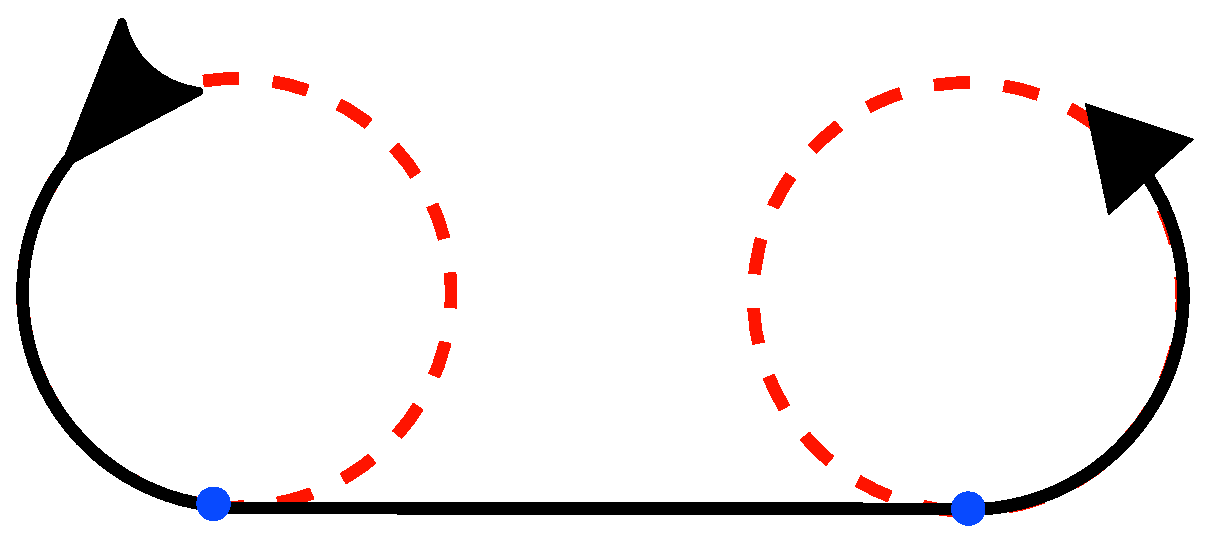
\includegraphics[width=0.5\textwidth]{WaypointDubins}
\caption[Commanding a Dubins path turn using waypoint navigation]{Using the existing waypoint navigation system to command a Dubins path turn}
\label{fig:waypointdubins}
\end{figure} 

Another alternative that was considered was to leverage the loitering capabilities of ArduPlane to command left and right hand turns. An example of how this would work can be seen in \ref{fig:loiterdubins}, where we place a waypoint at the centre of the circle formed by the extended arc we intend the UAV to travel . The issue seen with this would be that we would have to ensure that the UAV was in exactly the correct place when commanded to start the loiter segment, or else we would introduce irregularities into the path that would extend the length of the path and potentially throw off the entire process and cause the UAV to miss the virtual target intercept. Also, we would need to update the waypoints in much the same way as for the solution proposed in Fig. \ref{fig:waypointdubins}.

\begin{figure}[htbp!] 
\centering    
\includegraphics[width=0.5\textwidth]{LoiterDubins}
\caption[Commanding a Dubins path turn using loiter navigation]{Using the existing loiter navigation system to command a Dubins path turn}
\label{fig:loiterdubins}
\end{figure} 

Both of these solutions were considered too risky to attempt for this project, but could potentially provide excellent results if implemented correctly. By using the pre-existing navigation techniques we would by default be providing a method to correct cross-track error and as such more accurately track the desired path. However, as the path itself would be being regularly updated to counter the effects of wind, it is hard to know exactly how the UAV would behave. Deeper understanding of the ArduPlane navigation code would be required, or failing that just trying to implement this would tell us how they would perform.  

\subsection{Proposal 3: Plan} 
\label{future:alternatedubinsplan}

Both of these solutions would require changes to the default navigation system, both for loitering and for straight line following. The need to update the waypoint location could result in paths that are not smooth, negatively impacting battery usage and requiring frequent control inputs to the UAV, further increasing the risk of generating cross-track error. An alternative to this would be to find some way to define the waypoints as air relative locations, removing the need to update their position. This could be done if we have accurate values for the wind speed on board the UAV by calculating our position relative to the air using the GPS location and the wind values. 

Regardless of the approach used, this would be a very large undertaking, one which was considered too large and too risky for this project. Implementation and simulation would be the only true test of its performance however, making it hard to speculate on its benefits.

\subsection{Proposal 3: Summary} 
\label{future:alternatedubinssummary}

This proposal would be difficult to implement, as it is hard to know the exact location of the UAV relative to the air. Airspeed sensors would need to be combined with knowledge of the environmental factors to provide accurate location data, which could then be used as part of a navigation system. Also, this would require airspeed sensors on the UAV which would be additional to the minimum requirements to fly a UAV using ArduPlane.

We would also need to ensure that any paths generated from a moving waypoint would either be generated as smooth lines, or have them smoothed via some mathematical process, some form of spline function perhaps.

%******************************************************************************************************
%******************************************************************************************************
\section{Proposal 4: Planning Paths Onboard the UAV} 
\label{future:onboard}

Currently our system plans our new turns entirely on the ground. If we are able to calculate our paths on the UAV, it would allow us to better handle disturbances by wind.

\subsection{Proposal 4: Justification}
\label{future:onboardreason}

When we plan our paths we need to know the orientation of the UAV when starting the turn, as well as when we finish it. If we imagine a scenario in which we are reaching the end point of an imaging path and we need to start our turn, it is possible that a gust of wind has blown us off course or altered our orientation. By calculating the path when we are about to reach the start point of the turn, we can instead use accurate values for our orienation and as such plan a more suitable path. 

Further to this, if the wind speed increases or changes direction, we would be able to plan a new route to handle these changes, resulting in better alignment with the imaging path and providing higher quality aerial photographs. 

\subsection{Proposal 4: Plan} 
\label{future:onboardplan}

Our first consideration for this work would be whether the hardware currently available would be suitable. As discussed in Chapter 1, the APM boards do not have the storage capacity for even the latest stock versions of ArduPlane, so would definitely not be able to accommodate an additional feature such as this. The Pixhawk board may be able to, but this would need to be investigated beforehand. Another consideration is processing power; the current algorithm is a form of search algorithm, and depending on the input parameters may take a little while. The processors on both the Pixhawk and the APM are not massively powerful, so processing time would need to be a consideration. 

One solution to this would be to introduce some dedicated hardwre to handle the task. We could add an additional processor that could be connected up to the controller board and sensors which would then be solely responsible for calculating Dubins paths for the autopilot to use. Although this would introduce additional costs and weight to be carried, it would ensure that calculating these paths would not slow down the navigation systems or hog the processing power of the controller board.

With regards to the software itself, if we were to provide additional hardware, the only thing we would need to do would be to port it to the new device and configure it to take its inputs from the autopilot. If we were integrating it to ArduPlane, the process would be even easier, simply passing variables from within the autopilot system itself without the need to enable communication protocols or sensor connections. 

It may prove necessary to define a new processing algorithm to find a suitable Dubins path. Currently, we attempt to solve each of the Dubins path types for each set of inputs and then see if they meet our virtual target intercept criterion. If there was some way to simplify this process so that we were not assessing all 6 path types for each iteration of the algorithm, it would reduce the time taken to find a solution, and thus reduce our processing requirements. Currently the author is unaware of any such solution, so further investigation would be required.

\subsection{Proposal 4: Summary} 
\label{future:onboardsummary}

This is another proposal that could generate real performance improvements, and take the current solution one step closer to a system that would be suitable for operation in any wind condition. Calculating the paths on the UAV would introduce additional demand on processing, however the performance improvements we could expect may be worth any hardware investments to some users. One of the major drawbacks of the current system is its inability to handle the effects of wind gusts; this proposal would allow just that. 

%******************************************************************************************************
%******************************************************************************************************
\section{Proposal 5: Improving Handling of Gusts of Wind} 
\label{future:gusts}

As briefly touched upon in Proposal 2 (section \ref{future:tolerance}), this proposal aims at improving the systems ability to correct for perturbations due to gusts of wind. Again this is an improvement to performance, in particular to improve system reliability. 

\subsection{Proposal 5: Justification}
\label{future:gustsreason}

The ability to correct cross-track error generated by gusts of wind is important in any UAV navigation system, as gusts are unpredictable in both magnitude and duration. If we are able to correct disturbances from gusts during our new type of turn, we can ensure that we are correctly aligning the UAV with the imaging path as desired. This can help us to both improve battery usage by ensuring we take the most suitable path, whilst also helping to ensure high quality aerial images are captured by guaranteeing the UAV aligns with the next imaging path. 

The navigation system currently in use in ArduPilot has the ability to correct disturbances and reduce cross-track error, but the current implementation of our turning mechanism does not. 

\subsection{Proposal 5: Plan} 
\label{future:gustsplan}

In order to implement this proposal we would need a way to better define the path segments that the UAV is following. As it currently works, the UAV has no knowledge of the overall shape of the Dubins path we are commanding it to follow, only which direction to turn (L, R, or S) and for how long. In this respect, the work proposed in Proposal 3 (Section \ref{future:alternatedubins}) would solve this issue. 

Another solution would be to calculate the ground relative path for the UAV to follow, and to use a similar navigation system as is currently in place to follow it. This would require considerable changes to the current path planning software, as it would need to introduce curved paths that are calculated as a feature of wind. Our work so far provides a means for us to calculate these routes, but no way for us to define it within the mission plan. Currently, the mission plan for an ArduPlane mission is not capable of defining curved paths, except for as loiter paths, so work would need to be done in this regard. The navigation system in place currently calculates cross-track error by comparing the GPS position of the UAV with the vector between the previous waypoint and the next waypoint, which is of course represented by a straight line. In order for the UAV to recognise curved paths, we would need information included in the mission plan to define these curves to enable us to calculate and correct cross-track error. 

As mentioned, the completed work on this project provides us with a method for plotting a complex curved path in the form of a matrix of co-ordinates. Although it is not complicated to collect this data, it would be difficult (if not impossible) to load it all onto the UAV. A potential solution would be to limit the number of values in order to create a series of very short lines connecting a large number of waypoints, which when flown would essentially form a curve. This may be possible on the Pixhawk board as it is capable of storing a large number of waypoints, but would limit the maximum size of any mission implementing this technique. Further research into the viability of this work would need to be conducted.

\subsection{Proposal 5: Summary} 
\label{future:gustssummary}

For us to be able to correct cross-track error we need a new method for defining our Dubins paths. This would be a very large undertaking but could result in massive improvements in performance, stability, and resilience to environmental factors. The work completed in this project would provide a great starting point for this work, but would require a complete redesign of all of the changes made to ArduPlane for it to work.

%******************************************************************************************************
%******************************************************************************************************
\section{Proposal 6: Extending Path Planning to Work in 3D} 
\label{future:3d}

This final proposal is aimed at extending the range of applications for which we can use our new Dubins path turning mechanism. It would not improve performance, but instead add additional functionality that may prove useful in a number of photogrammetry scenarios.

\subsection{Proposal 6: Justification}
\label{future:3dreason}

In its current form, our system enables improved turning for aligning with imaging paths in only the 2D plane. If we wanted to fly at different altitudes for adjacent imaging paths we would need to add in additional waypoints to first alter our altitude, and then align with the next imaging path. If we were able to incorporate an altitude change into our current system, we could improve battery usage for any aerial photography usage requiring altitude changes. This would be particularly useful when surveying any area which displays large changes in elevation such as steep hillsides, mountains, or glaciers. By incorporating this change we would be able to keep a consistent relationship between a given area on the ground and the number of pixels that show that area. This means that once captured, the images would be able to be stitched together and display consistent resolution, removing the need to edit our collected images.

\subsection{Proposal 6: Plan} 
\label{future:3dplan}

Research documented in \cite{beard2013implementing}, \cite{hota2010optimal}, and \cite{lin2014path} show that this proposal is not only possible, it is effective too. Using the current navigation system available in ArduPlane, it would not be too much extra work to include our third axis of movement, whereby controlling for pitch changes could be carried out at the same time we alter roll and yaw. As with the current system, we would need to include allowances for disturbances and error due to wind and gusts, but in essence the navigation system would be relatively unchanged. The current waypoint navigation system accounts for changes in altitude, so if it was extended as proposed in Proposal 5, it would also be able to correct errors in $z$ axis. 
%TODO polish off this section

\subsection{Proposal 6: Summary} 
\label{future:3dsummary}

As with all of the proposals so far, this of course an element of uncertainty in regards to the effectiveness of this change. Whilst it would of course be a very useful change, if someone were to extend on this work of this project, this would not be the highest priority task moving forward. The actual changes to the path planning would not need to be too vast, we currently have three new commands relating to this project; turn left, turn right, and go straight. Adding 3D Dubins path turns would require us to specify a pitch angle too, however this could simply be included in the existing MAVLink commands and used when carrying out the regular commands. All in all this feature would not be too much extra work and would definitely improve the usefulness of this project, particularly as using UAVs for mapping unforgiving terrain is an attractive prospect and this proposal would help us to do so.

%******************************************************************************************************
%******************************************************************************************************

%!TEX root = ../MEngProject.tex

%******************************** Sixth Chapter *******************************************************
%******************************************************************************************************

\externaldocument{{../Chapter1/chapter1}}
\externaldocument{{../Chapter2/chapter2}}
\externaldocument{{../Chapter3/chapter3}}
\externaldocument{{../Chapter4/chapter4}}
\externaldocument{{../Chapter5/chapter5}}
\externaldocument{{../Chapter7/chapter7}}
\externaldocument{{../Appendix1/appendix1}}
\externaldocument{{../Appendix2/appendix2}}
\externaldocument{{../Appendix3/appendix3}}
\externaldocument{{../Appendix4/appendix4}}
\externaldocument{{../Appendix5/appendix5}}
\externaldocument{{../Appendix6/appendix6}}
\externaldocument{{../Appendix7/appendix7}}


% **************************** Define Graphics Path **************************
\graphicspath{{Chapter6/Figs/}}



%******************************************************************************************************
%******************************************************************************************************
\chapter{Project Planning and Management}
\label{planning}

This chapter will discuss the planning techniques used throughout this project, as well as discussing some of the problems encountered and overcome. Included in this chapter is a brief risk assessment which details how potential risks to the project were mitigated.



%******************************************************************************************************
%******************************************************************************************************
\section{Agile Planning}
\label{planning:agile}

As this project was entirely software based, there was some choice in the planning techniques available. The methodology employed was that of agile development, chosen for its flexibility, adaptability, and due to the author's familiarity with the process. From the beginning it was clear that it would be hard to provide time estimates for a number of tasks, due to working with an already established code base. By using an agile methodology it was possible to plan based on features rather than time allocation, which provided a level of flexibility necessary to deal with the levels of uncertainty resulting from extending the work of others. 

As our two tasks discussed in Chapters \ref{task1} and \ref{task2} were distinct from one another, so were the planning processes. As such, they shall be discussed separately.

As this project was an independent endeavour certain aspects of the traditional agile process were excluded, including stand-up meetings and retrospective meetings. By treating the project supervisor as both the customer and as a stakeholder, we still ensured regular meetings to discuss progress and features. These meetings provided a means to keep the project progressing in the correct direction by discussing planned features and how they fit into a finished product.

With regards to the planning, each of the two main tasks was treated as an ``Epic''. These epics were then broken down into ``Features'' and then further into ``User Stories''. This hierarchical design plan meant that the two epics could be worked on independent of one another, removing the need for a linear task-by-task approach. Fig. \ref{fig:AgileTree} shows how these tasks are structured. 

When using agile, a ``Spike'' occurs if there is a point at which research or investigation needs to be completed before other work can progress. Spikes were only used in this project to define research or investigation that occurred once other practical work had started, and as such research and the literature review completed before the project proper do not qualify as spikes.

\begin{figure}[htbp!] 
\centering    
\includegraphics[width=0.8\textwidth]{AgileTree}
\caption[Agile planning task breakdown]{A display of the hierarchy of tasks used in agile planning}
\label{fig:AgileTree}
\end{figure} 


\subsection{Agile Planning: Path Planning}
\label{planning:agile:planning}

The first step for this task was to define the epic that was being worked towards to serve as the overall aim for the task. After some consideration and discussion with the project supervisor, the Epic was specified as

\begin{displayquote}
	``To provide a path planning utility to enable a user to plan a turn using a Dubins path, in the presence of wind''
\end{displayquote}

This epic was then described via a number of product features, which were:
\begin{enumerate}
	\item Produced Dubins paths can be described as three distinct segments, using turning direction and segment length
	\item The user can calculate a Dubins path based on a series of inputs relevant to their UAV usage scenario
	\item The system can calculate the effects of wind on the travelled path, and compensate for it
\end{enumerate}

We are able to treat each of these features as iterations in the scope of this project. Strictly speaking this may not be correct for the agile methodology in an industry setting, however because this work was being completed by one person, testing could not be carried out concurrently with development. As such, each feature was implemented and tested before moving on to the next feature, thus they have been treated as iterations. Where necessary, re-factoring was performed when testing failed or highlighted problems. After re-factoring testing was repeated before moving on to the next iteration.

Continuing on from their definitions, each feature was further described using one or more user stories:

\begin{table}[h!]
\centering
\caption{The breakdown of features into user stories for the path planning task\label{tab:task1planning}}
 \begin{tabular}{p{0.4\textwidth} | p{0.5\textwidth}}
	\hline
	\textbf{Feature} & \textbf{User Story} \\
	\hline
	\hline
	\multirow{2}{0.4\textwidth}{Produced Dubins paths can be described as three distinct segments, using turning direction and segment length} & As a user, I am informed of the Dubins path type because it is information I need to edit a mission plan \\
	\\
	& As a user, I am informed of the length of each path segment because it is information I need to edit a mission plan\\
	\hline
	\multirow{3}{0.4\textwidth}{The user can calculate a Dubins path based on a series of inputs relevant to their UAV usage scenario} & As a user, I am able to specify the speed and turning radius of the UAV because I need to cater to the UAV platform I am using\\
	\\
	& As a user, I am able to specify the speed and direction of wind because I need the system to consider the wind where I am flying my UAV\\
	\\
	& As a user, I am able to specify the start and end locations and orientations so that I can generate a suitable path\\
	\hline
	\multirow{2}{0.4\textwidth}{The system can calculate the effects of wind on the travelled path, and compensate for it} & As a user, I can specify a desired ground-relative end point, and be presented with the air relative Dubins path necessary to reach it, because I do not have accurate knowledge of the offset the wind will generate\\
	\\
	& As a user, I receive Dubins paths for flight to a destination both with and without the effects of wind so I can examine the impact of wind on the flight path and battery requirements\\
	\hline
 \end{tabular}
\end{table}

These user stories were satisfied by the console application produced, irrespective of the failings of the system as a whole. We can imagine the user stories listed here as comprising the first release of the path planning system, as once complete they offer a complete system with which the user can interact. If time had permitted, the next release for this system would have integrated it into either APM Planner 2 or MissionPlanner. This would have have been a most agreeable addition that would have massively reduced the time required to test the system, as creating mission plans would have been straightforward and not required manual editing of mission plans. However this was not planned out during the project, as that would have represented planning the next release before the current one was complete, which would be at odds with the methodology in use.

As previously mentioned, the aim of using this planning style was to organise the project via features and functionality, rather than by time. In this respect it proved very beneficial, as no hard deadlines were placed on the work, instead the product was considered complete once all of the features were implemented. 

\subsection{Agile Planning: Path Following}
\label{planning:agile:following}

The epic for this task must reference the integration of the solution with the path planning solution, as without it this task is relatively meaningless. The epic itself is in fact very simple, and reads

\begin{displayquote}
	``To implement changes to ArduPlane to allow it to fly a Dubins path''
\end{displayquote}

With this short description we are able to regard this task as independent, yet related to the path planning task. The mention of Dubins paths signifies its interaction with the path planning solution, however does not imply it as being absolutely necessary to this task.

As touched upon in Chapter \ref{task2}, the current implementation was not the first implementation attempted. As such, it was not the first planned implementation, meaning that the planning information presented here was not the first planning information generated. Thus, the features and user stories here were the ones used to implement the final solution, but have changed over time. This is another benefit of the agile methodology, as when problems were encountered, the plan was quickly adapted to suit the needs of the project. 

The features derived from the epic are as follows
\begin{enumerate}
	\item ArduPlane must recognise control messages and commands relating to flying a Dubins path
	\item ArduPlane must navigate according to the new control messages to perform a Dubins path turn
	\item The implemented changes must not negatively impact the pre-existing navigation systems of ArduPlane
\end{enumerate}

As before these features have been treated as iterations. And once again we can look at these features more closely by expressing them as user stories@

\begin{table}[h!]
\centering
\caption{The breakdown of features into user stories for the path following task\label{tab:task2planning}}
 \begin{tabular}{p{0.4\textwidth} | p{0.5\textwidth}}
	\hline
	\textbf{Feature} & \textbf{User Story} \\
	\hline
	\hline
	\multirow{2}{0.4\textwidth}{ArduPlane must recognise control messages and commands relating to flying a Dubins path} & As a user, I want ArduPlane to recognise the commands I am issuing because they are necessary to navigate my UAV \\
	\\
	&  As a user, I want ArduPlane to recognise all of the commands required to fly a Dubins path because otherwise my UAV will not navigate to the right location\\
	\hline
	\multirow{3}{0.4\textwidth}{ArduPlane must navigate according to the new control messages to perform a Dubins path turn} &  As a user, ArduPlane must perform L,R, and S segments according to my commands so as to complete a Dubins path\\
	\\
	&  As a user, ArduPlane must perform these segments for the specified duration or else the Dubins path will not be useful to me\\
	\\
	&   As a user, ArduPlane must turn as instructed otherwise my UAV will not align with my imaging paths\\
	\hline
	\multirow{2}{0.4\textwidth}{The implemented changes must not negatively impact the pre-existing navigation systems of ArduPlane} &  As a user, automatic flight mode must still work, because the majority of my missions are flown in automatic mode\\
	\\
	&  As a user, new features must not regress the autopilot as a whole as I use it for a number of tasks other than aerial photography \\
	\hline
 \end{tabular}
\end{table}


Once more there were future releases in mind that were not able to be realised as a result of time constraints. The second release would have been a primarily re-factoring phase, with changes to both the path planning and following solutions being made as a result of simulator testing. Following this a tertiary release cycle was in mind, primarily aimed at testing the system on a real UAV as opposed to a simulated one. Changes would have been required on the path following system to adapt it to the flight characteristics of the chosen UAV.

\subsection{Previous Implementation Attempts}
\label{planning:agile:previous}

The previous attempts at solving the path following problem have not been discussed yet, but are worth mentioning here. The initial plan involved creating a ``DUBINS'' flight mode, which would be responsible for handling all navigation whilst performing a Dubins path turn. Although the new flight mode was successfully added, a number of problems arose when attempting to use it. The primary issue appeared when trying to switch to and from AUTO mode to the new flight mode. In doing so, the mission plan was not being read correctly and ArduPlane was detecting a problem and would return to its launch location. This is a fail-safe behaviour of ArduPlane that occurs when it determines no mission plan is currently active. After numerous attempts to enable the mission to continue via a range of techniques, this approach was abandoned and the approach described above was adopted.

%******************************************************************************************************
%******************************************************************************************************
\section{Problems Overcome}
\label{planning:problems}

Sadly, this project suffered greatly due to a number of unforeseen problems. Luckily, the path planning task was able to progress unhindered, with no major delays or setbacks, however the path following solution bore the brunt of these problems. 

The first major problem was encountered when attempting to build the ArduPlane code for the first time. It is still unclear why, but the instructions provided by the ArduPilot project for building the code on a Windows operating system were either incorrect or incomplete. Attempts were made to compile a wide range of ArduPlane versions, using a series of different tools and techniques. None of them seemed to work, no matter how much time was dedicated to it. The solution to this problem was to carry out the work on a Linux operating system; the distribution chosen was Ubuntu due to the author's familiarity with the platform. This change allowed the code to be compile by making use of Linux's ``make'' command, which compiled the code first time with no issues. 

Another problem arose as a result of ambitions for the direction of the project. As mentioned above, it was hoped that this project would eventually be tested on a real UAV, which would require the presence of a controller board. As mentioned in \ref{intro:hardware}, the two popular and readily available boards are the Pixhawk and the APM 2.x series of boards. In recent months the ArduPilot project has ceased to support the APM 2.x series of controller boards in favour of the more powerful Pixhawk boards. However, APM 2.x boards are still available for purchase, and slightly older version of ArduPlane are still compatible with them. Because of the large price difference between the two options, and the financial constraints on this project, it was decided that the base version to work from should be an older version of the code suitable for the APM boards. This was an attempt at forward planning in case the opportunity arose to test the system on a real UAV. 

There is documentation available on the ArduPilot developer wiki that can allow a user to build the code for a Pixhawk board using the Eclipse IDE when using a Windows operating system. However all documentation and attempts by the author to use an IDE to build the code on any platform failed miserably. As a result, the majority of the time spent working on the path following solution was spent developing using simply a text editor and the command line to build the code. This slowed down implementation massively, as the code base was large, complex, and highly genericized meaning that tracing the program flow was difficult. In addition, it was almost impossible to work out the call hierarchy for any function, due to the way in which generic libraries were utilised in ArduPlane.

Towards the latter stages of the project, it was realised that as time was running out, it was unlikely that a real-world test would be able to be carried out. As time was running out it was becoming very clear that the only solution was to find some way to get the code to build in a proper IDE. With a lot of perseverance, guess-work and a touch of luck, the code was able to be imported into Eclipse on Linux, even though there was no documentation online suggesting this was possible. One change that was necessary to make however was to move to a slightly different version branch, which meant a number of changes needed to be re-added, using up yet more time. 

The change to a new version was important, as the new branch being used had been released after the ArduPilot project had moved away form their Arduino based roots to a more C\texttt{++} dominant implementation. It was this change that enabled the compilation of the code in Eclipse, as previously a large proportion of the code was implemented in Arduino-based \textit{.pde} files, which Eclipse did not work well with.

The final issue worth discussing was encountered with the simulator; contrary to instructions available online \cite{ArduPilotSITL}, the simulator measures wind in feet per second, not metres per second. This meant that for a long period of time, simulations that were intended to have a 5 metres per second wind were in fact being carried out with a 1.5 metres per second wind. The confusion following this wasted yet more time.

In summary, this project was plagued with delays. As discussed throughout the report, it was well known from the planning stages that the solution being implemented would not be perfect. The initial thinking was that it would be relatively straightforward to implement this system and then build on it and adapt it to improve performance. Due to the sheer number of setbacks and unfavourable platform issues, there simply was not enough time to do so. It is a great shame, as this project had a lot more potential than was displayed.

%******************************************************************************************************
%******************************************************************************************************
\section{Risk Management}
\label{planning:risks}

Throughout the project there were a number of potential risks identified and taken into consideration. The following table lists these perceived risks, the negative impact (on a scale of 1 - 10) on the project should they have occurred, and steps taken to mitigate these risks: 

\begin{table}[h!]
\centering
\caption{Risk assessment breakdown for the project as a whole\label{tab:riskassessment}}
 \begin{tabular}{p{0.3\textwidth} | p{0.1\textwidth} | p{0.4\textwidth}}
	\hline
	\textbf{Risk} & \textbf{Impact} & \textbf{Mitigation} \\
	\hline
	\hline
	Loss of code & 9 & Use of file versioning system ``git'' alongside remote storage on GitHub massively reduces the risk of this occurring. In addition, local copies were regularly updated on two different computers \\
	\hline
	Injury whilst testing real UAV & 4 & Although this would have been terrible, it would not necessarily have impacted the project itself all that much. Regardless, this risk never had to be mitigated as real-world testing was never completed \\
	\hline
	Failure to deliver solutions to one or both of the tasks for this project & 7 & The impact would be considerable, as failure to deliver any solution would be regrettable. A solution with flaws would be preferable. To mitigate this, the planning process ensured that with enough time allocated to the work, at the least some minimal solutions would be created \\
	\hline
 \end{tabular}
\end{table}

With all things considered there were very few genuine risks to this project. That being said, it did fall foul of one of the risks listed above. Early on in the project, git was being used with a relatively new front-end user interface, so as to easily visualise progress and branch hierarchies. This front-end product was in beta, however had received a number of positive review online. Due to some unknown communication error, a number of commits to the code were never pushed to the remote repository, and the program locked up. Not noticing that the changes had not been pushed, the author switched to using command line git as the front-end interface was not all that useful after all. In the process of uninstalling the program, these commits were somehow lost, and along with it a fair amount of code. Luckily this was early on, so not a huge amount had been implemented, and the changes to ArduPlane were successfully re-implemented.

%******************************************************************************************************
%******************************************************************************************************
\section{Project Planning and Management Summary}
\label{planning:summary}

On the whole, the planning conducted was both effective and and flexible. The flexibility of this approach proved its worth after coming up against a number of setbacks, delays, and difficulties. In retrospect, the planning stage was not thorough enough and not specific enough. A better approach would have been to dedicate a period of time for a series of spikes and investigations before attempting to plan the features of the product. One of the mistakes was rushing to start implementation merely accepting that the working environment was far from ideal, by just working in a text editor. If more time had been spent experimenting with possible IDE solutions, a large amount of time could have been saved and the finished products may have been more advanced. 

Another slight failure in the planning phase was not dedicating enough time devoted solely to writing this report. As with any report writing, the time required to complete it was longer than expected, meaning the finished version is not quite to the level the author would have desired. Nonetheless, the author feels it is thorough and complete, just that it could have been a little more elegant in places.

With the beauty of hindsight, one can imagine a slightly different series of events having unfolded. If the path following changes had been implemented before the path planning, the true roll behaviour of the UAV would have been evident earlier on in the project. This could have meant that a suitable path planning model could have been used in its first iteration. This would have been excellent, but the problems encountered when working with the ArduPlane code would most likely have prevented this from becoming a possibility. 

To summarise, this project has been a real test. The practical work required a lot of flexibility and adaptability, due to both unforeseen problems and the requirement to work with pre-existing products. Overall the work itself has been a success, however the final products a failure. Every failure is a lesson though.
%******************************** Seventh Chapter *****************************************************
%******************************************************************************************************

\externaldocument{{../Chapter1/chapter1}}
\externaldocument{{../Chapter2/chapter2}}
\externaldocument{{../Chapter3/chapter3}}
\externaldocument{{../Chapter4/chapter4}}
\externaldocument{{../Chapter5/chapter5}}
\externaldocument{{../Chapter6/chapter6}}
\externaldocument{{../Appendix1/appendix1}}
\externaldocument{{../Appendix2/appendix2}}
\externaldocument{{../Appendix3/appendix3}}
\externaldocument{{../Appendix4/appendix4}}
\externaldocument{{../Appendix5/appendix5}}
\externaldocument{{../Appendix6/appendix6}}
\externaldocument{{../Appendix7/appendix7}}

\chapter{Conclusions}
\label{conclusion}

% **************************** Define Graphics Path **************************
\graphicspath{{Chapter7/Figs/}}


%******************************************************************************************************
%******************************************************************************************************
\section{Conclusions}
\label{conclusion:conclusion}

There has been a great deal learned throughout the course of this project with regards to both UAV flight planning, open source software products, and the ArduPilot project itself. It is a great shame that the project suffered so many setbacks, as with a bit more time, a more suitable path planning solution could have been developed which may have changed the findings of this report considerably. The final results were both disheartening and frustrating, as the ideas behind this project show promise but have not been able to be fully realised. 

As mentioned time and time again, it was well known prior to making any changes to ArduPlane that the path planning solution was not completely fit for purpose. As the work being conducted involved so many unknown factors (primarily the behaviours of ArduPlane and the UAV being simulated), the attempt to ``try it and see'' may have proven successful given more time. If the path planning application were modified to better consider the true turning behaviours of the UAV however, it definitely has potential to meet all of the requirements laid out for aligning with imaging paths. A more finalised solution will not be able to make use of ``true'' Dubins paths, although a slightly modified version that lengthens turning arcs where necessary may prove very effective. By calculating a turn based on a Dubins path but with allowances and tolerances for the roll rate of the UAV, the changes made to ArduPlane could be leveraged to form a thorough and comprehensive solution to the problem discussed here. Perhaps this work will be conducted at some point in the future; its a nice thought at least.

The changes made to ArduPlane, whilst admittedly rudimentary, served their purpose and fulfilled all of the user stories planned out. In some regards the additions to ArduPlane were in fact perfect; they met the requirements in the simplest possible way, without compromising any of the pre-existing behaviours of the autopilot. If this work was to be continued with the aim of incorporating it into an official version of ArduPilot, not all that much would need to be changed in the ArduPlane code. By performing banked turns using the UAV's own roll limits, the solution implemented is in theory suitable for any UAV which may be using ArduPlane. Of course further testing on a range of platforms would be required to verify this, although it is hard to imagine why this would not be the case.

The problems faced throughout this project have been numerous, irritating, and often tricky to overcome. The open-source nature of ArduPlane and the fact that over recent months it has undergone very large changes to its codebase are two features that have combined to create whole problems of their own. As the developers behind the project are not working on this for financial gain, there is little incentive to produce thorough and detailed documentation. The result of this has been a lot of failed attempts at various tasks based on incomplete or unsuitable documentation. The number of problems that were also addressed via forum posts is also worrying; although the community involved in this work is clearly very knowledgeable, it doesn't inspire confidence when cobbling together solutions from a variety of posts on a number of topics.

There have however, been two mistakes that are clearly mistakes and should have been addressed sooner. The decision to try and work on an older version of the product, simply with the intention of reducing the cost of any purchased hardware, was clearly misguided. In retrospect this project should have started out with the latest version of the code from the get-go, not least because the latest versions are almost entirely C\texttt{++}, as opposed to the unholy combination of C, C\texttt{++}, and Arduino files which comprise the older version of the product. The second mistake was a result of stubbornness; progress should have been shelved and greater efforts made to build the code in an IDE much sooner. In fairness however, there was no documentation nor forum posts that suggested getting the code to build in Eclipse on Linux was even a possibility. 

When all is said and done, the behaviour of stock ArduPlane is not ideal, however it far outperforms the current version of this new path planning and following system. It would be nice to see further work completed on this project, as even an extra few weeks could create something great. Who knows, it could even lead to a real UAV flying using this code!




\end{mainMatterEnv}

% Back Matter
\begin{backMatterEnv}


% Glossary
\printglossaries

% \printbibliography

\bibliographystyle{IEEEtranOnlineMod}
%\bibliographystyle{IEEEtran}
\bibliography{IEEEabrv,references}

% Appendix
        \begin{chapterEnv}[appen:loads]{Load of Appendices}
            \begin{sectionEnv}[asec:example-appendix]{An Appendix}
                Example appendix!
            \end{sectionEnv}
        \end{chapterEnv}


\end{backMatterEnv}

\end{document}


